\documentclass[11pt]{article}

\usepackage{graphicx}
\usepackage{caption}
\usepackage{amsfonts}
\usepackage{xcolor}
\usepackage{subfig}
\usepackage{subfloat}
\usepackage{hyperref}
\usepackage{eurosym}

\graphicspath{{IMG/}}
	
\begin{document}
    \raggedbottom
    \sloppy \lefthyphenmin=1000
    \setlength{\parskip}{3ex}

\title{NEW Infrastructures and Risk assessment overview \\Executive Summary}

\author{J. Toledo}


\maketitle

\section{Scope and outlook}

The present document provides an summary of the status of the infrastructures and the risk assessment for the NEW detector.

Throughout the risk assessment review, the NEXT Collaboration request permission to the LSC to operate the NEW detector with Ar and depleted Xe, 
with pressure in the vessel in the range 5-10 bar. After a period of operation, the Collaboration will  request permission to operate with enriched Xe, which will imply a new risk assessment process.
 

\section{Hazards associated to NEXT infrastructures}
NEXT occupies the far end of the Hall A. A supporting structure with tramex floor delimits the 11x11 m2 NEXT experimental area and working platform. 
Under the platform, and covering most of Hall A extension, a large pool exists to protect personnel from gas and liquid dumps.

\begin{itemize}
\item Gas venting and asphyxiation hazard: the amount of Xe liberated in a catastrophic failure would be less than 1.5 m3 and it does not represent any asphyxiation hazard, given its small volume compared with the total volume of the experimental hall and the presence of the pool, where gas 
(Ar and Xe are heavier than air) will sink  to a thickness of less than 1 mm.
\item Seismic hazard:A seismic structure, designed according to national regulations and approved by LSC, occupies the center of the working platform. The NEW vessel and lead castle are mounted on top of the pedestal. The structure is described in detail in the companion document Seismic_report.pdf, "NEXT-100 project: Structural Seismic Analysis",  Release 1.0 October 17, 2012.
\item Hazards related to the lead castle: A safe operation protocol for the opening and closing the the castle, approved by LSC, can be found in Process Procedure NEXT-NEW-001 (Process Procedure: Opening and closing the NEXT experiment lead castle).
\item Hazards related to liquids: Only two potentially hazardous liquids are used in NEXT, the ethylene-glycol (20-30\% in volume in the chiiler and the liquid nitrogen used in the cryo-recovery bottle only when a cryo-recovery operation is to be carried out. LSC has a well defined safety procedure for the use and handling of liquid nitrogen in the laboratory, which we will follow (LSC's document "Instrucciones de operaci\'on y seguridad NITROGENO LIQUIDO.pdf".
\end{itemize}


\section{Hazards associated to equipment on the NEXT platform}
Hazards associated with the Gas System (NEW vessel, recovery talk, compressor, chiller, recirculation circuit, cryogenic recovery bottle and a number of manual and pneumatic valves) 
are described in more detail in document "Process Procedure NEXT-NEW-009: Operation methods and procedures relating to NEW Gas System", as well as in a number of analysis documents 
for the Gas System (FMECA analysis and report, Fault Tree Analysis, Fatigue analysis and Criticality analysis). 
A HAZOP analysis has been carried out by Insegma (www.insegma.com) in March-April 2016 (report to be released in April 2016).

Hazards associated with the electronics (Energy Plane rack, Tracking Plane rack, DAQ Computing rack, Very High Voltage rack, Slow Controls, and UPS units) are addressed in 
"Overview of the Risk Assessment for Electronics in the NEW detector" and more specifically in the FMECA table and report 
files. 

\subsection{Issues related to NEW vessel}
The NEW vessel is a tank with a volume of 0.169 m3 made of 316Ti material and with CE certification at 20 bar and vacuum. The main issues associated with this component is a vessel rupture due to overpressure or a gas leak due to material fatigue or o-ring breach. 
The use of bursting disks and an automatic venting to the emergency recovery tank mitigate the risk of overpressure.

In the unlikely case that a vessel rupture provokes an explosion, which is the only hazard for personnel associated with the NEW vessel, the castle acts as a shield.

\subsection{Hazards with other components in the Gas System}
The recovery tank for NEW is the NEXT-100 vessel (volume of 2,558 m3 made of 316Ti with a CE certification at 15 bar). 
It is kept at at 10-5 mbar during normal operation. The size of the tank ensures that after an emergency recovery situation the final absolute pressure is in the order of 1 bar. Thus, this component poses no hazards to the LSC installations or to personnel. Still, a bursting disk (BD1) prevents excessive 
pressure in the tank.

The cryo-recovery bottle has a volume of 0.060 m3. It is made of 316Ti and has CE certification at 130 bar. It is mounted on a base firmly screwed to the tramex floor.

Hazards related with this component are (1) damage to personnel due to an accident handling of the liquid nitrogen, (2) explosion due to material fatigue or overpressure. 
The former requires to follow LSC's liquid nitrogen handling protocol. The latter is mitigated by the presence of bursting disks.

The getters pose no hazards for personnel or LSC infrastructures. The same can be said of vacuum pumps 1, 2 and 3. The hot getter is self monitoring. It will shut down in the event of a detected fault and the gas flow will be re-directed through an internal by-pass line. The cold getters are passive and need to be replaced when the captured impurities reduce the gas flow (a piece of software monitoring pressure gauges PG5 and PG6 can give a hint on when the getters are to be replaced).


The role of the compressor is to move the gas through the purification loop. It is a very reliable device having triple diaphragms to compress the gas. 
In case of diaphragm breach, hydraulic oil leak or other failures detected by the built-in monitoring system, the compressor will be automatically turned off and isolated from the gas system. 

The compressor needs external cooling, so a chiller unit will remove heat through a heat exchanger. A failure in the chiller will also turn off and isolate the compressor. 

The regulator bottles with pressure gauges are used to fill the gas system with Ar or Xe to a desired pressure. 
Pressure gauges on both ends of each regulator, as well as in other points of the circulation loop, together with a well defined protocol (see Initial fill procedure in NEXT-NEW-009) minimize the risks of overpressure, which is the main hazard for this set of components. 


\section{Safety procedures and risk assessment for NEW}
Several Process Procedures have been written to address specific operations in NEW commissioning and operation, describing hazards and defining safe working procedures. 
All of them have been approved by LSC.

Four new Process Procedures are being produced, to address the commissioning and operation of the field cage's high voltage, the use of radioactive sources and the commissioning and operation of the Gas systen in NEW. These Procedures will cover the range of (currently) intended operations.

\begin{figure}[ht!]
    \bigskip
    \begin{center}\leavevmode
        \rotatebox{0}{
        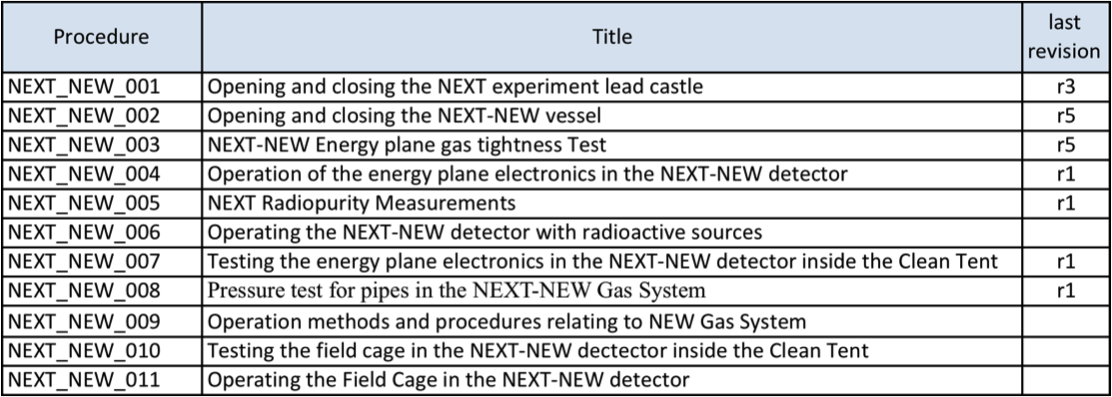
\includegraphics[width=\textwidth, ]{Procedures.png}}
        \caption{\textit{List of existing and in-preparation NEXT NEW Process Procedures}}
        \label{fig:PROC:PROC}
    \end{center}
\end{figure}


A risk assessment review took place at LSC on 8th and 9th February 2016, organized by the LSC Director and counting with 6 experts from LNGS in the review panel.
The documentation (FMECA analysis, quantitative criticality analysis and a description of the gas system elements and operation, among other documents) as well as NEXT'w working 
platform were reviewed.

Although no major problems were detected, a number of enhancements in the gas system design were suggested. 
Additionally, the panel advised to (1) carry out a HAZOP analysis leaded by an external company, (2) do gas flow calculations for the critical elements and 
(3) enhance the technical drawings for the gas system to adhere to the ISA Standard S5.1 Instrumentation Symbol Specification. 

A HAZOP analysis has been carried out with the help of the company Insegma (www.insegma.com) in March-April 2016. We are waiting to receive the final report, though we have already
used the analysis results to enhance the safety and reliability of the gas system.

The legalization of the Gas System is being prepared by an external company, Cryovac, who has carried out its own safety analysis and made requests and suggestions which have been already addressed.

Gas flow calculations have been carried out, validating the original design assumptions. The technical drawings are currently being updated to the ISA S5.1 standard.

Safety reviews at LSC, the one carried out by Cryovac and the HAZOP analysis by Insegma have been extremely useful to identify weak points and produce a better design and documentation. NEXT-NEW Process Procedure (Operating
methods and procedures relating to NEW gas system), which is to be submitted to LSC between 18th and 22nd April 2016, is the reference document for the gas system description and operation.

\subsection{Next steps}
LSC poses the following conditions to grant permission to operate the gas system with Argon and commercial/depleted Xenon between 5 and 10 bar: 
\begin{itemize}
\item Perform pressure tests for rigid pipes in the Gas system. Tests have been already carried out early in April.
\item Hand in the HAZOP analysis report and updated risk assessment documentation (including Process Procedure NEXT-NEW-009). The docuementation needs to be approved by LSC. NEXT will hand in these documentation in the third week in April.
\item Legalize of the pressure system according to national and regional regulations. The company Cryovac is taking care of this and the process should have concluded the last week of April.
\end{itemize}

Starting in May 2016, we plan to run, test and debug the detector throughout the rest of 2016. Learned lessons will allow us target operation up to 15 bar with enriched Xenon after the correspondign new risk assessment and, if applicable, gas system upgrade.



\end{document}




